\documentclass[aspectratio=169,11pt]{beamer}
\usepackage{teaching_slides}

\title[L9a - Panel Data]{ Econometrics I}
\subtitle{Lecture 8a: Panel Data and Fixed Effects}
\author{Chris Conlon \\NYU Stern}
\date{Fall 2026}

% New deck (Fall 2026). Readings: Hansen Ch. 17; Mixtape Ch. 8.
% All figures/tables are simulated with known ground truth: see panel_sims.R.
% In-class workbook: inclass_session8.Rmd

\newcommand{\iid}{\text{i.i.d.}}

\begin{document}
\maketitle

\begin{frame}{Where we are}
\begin{itemize}
	\item Weeks 5--7: identification by \alert{design} --- randomize, or find an instrument.

	\medskip
	\item Today: identification by \alert{repeated observation}. We see the same firm, store,
	customer, or state many times. What does that buy us?
	\begin{itemize}
		\item Part a (this deck): fixed effects, random effects, and the choice between them.
		\item Part b: event studies --- the panel version, and the earnings-announcement version.
	\end{itemize}

	\medskip
	\item The one idea: things about unit $i$ that \emph{never change} can be removed
	without ever measuring them.

	\medskip
	\item Readings: Hansen Ch.~17; Mixtape Ch.~8.
\end{itemize}
\end{frame}


\begin{frame}{What a panel is}
\begin{itemize}
	\item Units $i = 1,\dots,N$ observed at periods $t = 1,\dots,T$ (or $T_i$ if unbalanced).
	\medskip
	\item The panels you will meet are \alert{wide and short}: $N$ large, $T$ small.
	\begin{itemize}
		\item firms $\times$ fiscal years (Compustat: $N \approx 5{,}000$, $T \approx 10$--$40$)
		\item stores $\times$ weeks (scanner data)
		\item customers $\times$ months (subscription, churn)
		\item hospitals or physicians $\times$ quarters
	\end{itemize}
	\medskip
	\item Everything today is ``$N \to \infty$, $T$ fixed.'' Large-$T$ panels (countries, 50 years)
	are a different world: unit roots, cointegration, Nickell bias that goes away.
	\medskip
	\item Notation: $y_{it}$ outcome, $x_{it}$ a $k$-vector of regressors. Bars are unit means:
	$\bar y_i = T^{-1}\sum_t y_{it}$.
\end{itemize}
\end{frame}


\begin{frame}{The model}
\begin{align*}
	y_{it} = x_{it}'\beta + \alpha_i + \varepsilon_{it}
\end{align*}
\begin{itemize}
	\item $\alpha_i$: \alert{everything about unit $i$ that does not change over $t$}.
	Management quality, brand, location, a CEO's risk appetite, a customer's taste.
	\medskip
	\item $\varepsilon_{it}$: the idiosyncratic shock. Different every period.
	\medskip
	\item The conditional mean we want is $\E[y_{it} \mid x_{it}, \alpha_i] = x_{it}'\beta + \alpha_i$.
	The whole subject: what happens when you \emph{cannot} condition on $\alpha_i$?
	\medskip
	\item Two names for $\alpha_i$, and they are not synonyms:
	\begin{itemize}
		\item a \alert{fixed effect}: treat $\alpha_i$ as a parameter (or a nuisance) --- no assumption
		about how it relates to $x_{it}$.
		\item a \alert{random effect}: treat $\alpha_i$ as a draw, \emph{uncorrelated} with $x_{it}$.
	\end{itemize}
\end{itemize}
\end{frame}


\begin{frame}{Running example: management practices and productivity}
\begin{itemize}
	\item Bloom and Van Reenen (2007) score firms on management practices (monitoring, targets,
	incentives) and ask whether better practices raise productivity.
	\medskip
	\item The obvious worry: well-run firms adopt good practices \emph{and} are productive for
	other reasons. Firm quality $\alpha_i$ drives both.
	\medskip
	\item Our simulated version, with ground truth:
	\begin{align*}
		y_{it} &= 1 + \alert{0.10}\, x_{it} + \alpha_i + \gamma_t + \varepsilon_{it}, \qquad
		\alpha_i \sim N(0, 0.5^2),\ \varepsilon_{it} \sim N(0, 0.3^2) \\
		x_{it} &= 0.7\,\alpha_i + \text{(persistent firm component)} + \text{(year-to-year noise)}
	\end{align*}
	$N = 200$ firms, $T = 8$ years. $y$ is log productivity, $x$ the practices score.
	\medskip
	\item We know $\beta = 0.10$. Every estimator gets judged against that number.
\end{itemize}
\end{frame}


\begin{frame}{The picture}
\begin{center}
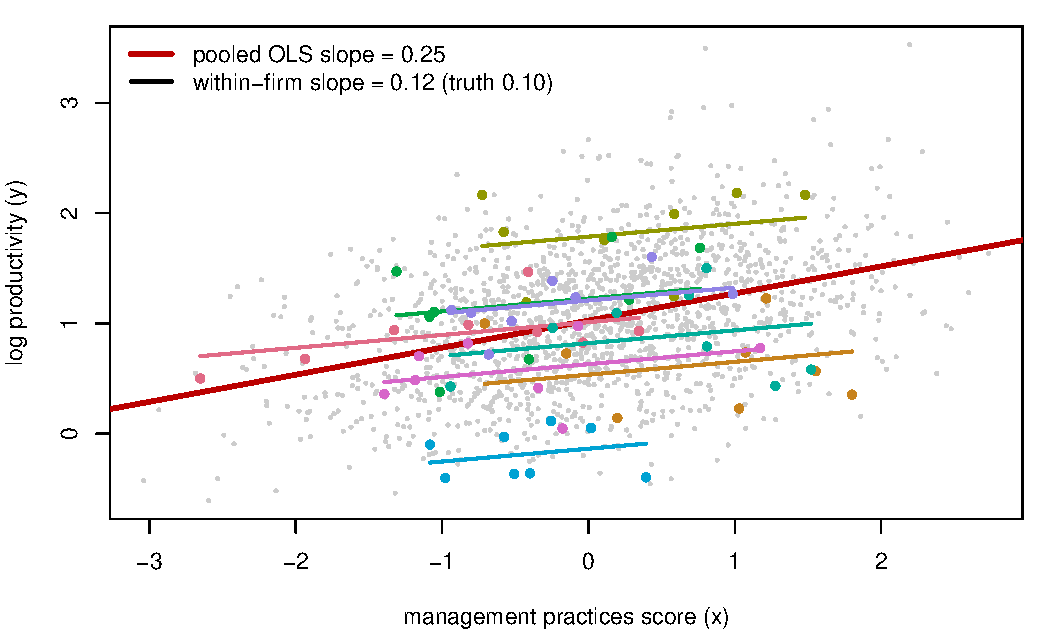
\includegraphics[width=.6\textwidth]{fig_mp_pooled_vs_fe.pdf}
\end{center}
\vspace{-.3cm}
{\small Grey: all firm-years. Colored: eight firms, each with its own within-firm fit. The pooled
line runs through the \emph{between-firm} cloud; the within-firm lines have the true slope.}
\end{frame}


\begin{frame}{Pooled OLS: when is it fine?}
Ignore the panel structure and regress $y_{it}$ on $x_{it}$ (and a constant).
\begin{align*}
	\hat\beta_{\text{pooled}} \xrightarrow{p} \beta + \frac{\Cov(x_{it}, \alpha_i)}{\Var(x_{it})}
\end{align*}
\begin{itemize}
	\item Same omitted-variable formula as Week 2. The omitted variable is $\alpha_i$.
	\medskip
	\item Consistent iff $\Cov(x_{it}, \alpha_i) = 0$ --- the ``random effects'' assumption.
	\medskip
	\item In the example, $\Cov(x, \alpha) > 0$: pooled OLS is biased \emph{up}. Good practices
	look more effective than they are because good firms have them.
	\medskip
	\item Even when unbiased, pooled OLS standard errors are wrong: $\alpha_i$ sits in the error
	of every period for firm $i$, so errors are correlated within firm. Cluster by firm (Week 3).
\end{itemize}
\end{frame}


\begin{frame}{Three ways to get rid of $\alpha_i$}
\begin{enumerate}
	\item \alert{Dummies (LSDV).} Put in $N$ firm indicators and run OLS. Fine for $N = 200$;
	awkward for $N = 5$ million customers.
	\medskip
	\item \alert{Within transformation.} Subtract the firm mean from every variable:
	\begin{align*}
		(y_{it} - \bar y_i) = (x_{it} - \bar x_i)'\beta + (\varepsilon_{it} - \bar\varepsilon_i)
	\end{align*}
	$\alpha_i - \bar\alpha_i = 0$. It is gone. OLS on the demeaned data is the \alert{fixed-effects (FE)
	estimator}.
	\medskip
	\item \alert{First differences.} $\Delta y_{it} = \Delta x_{it}'\beta + \Delta\varepsilon_{it}$.
	Also kills $\alpha_i$.
\end{enumerate}
\medskip
\begin{itemize}
	\item (1) and (2) give \emph{identical} $\hat\beta$ (FWL: demeaning is projecting off the
	dummies). (3) equals them when $T = 2$; differs otherwise.
	\item All three use only \alert{within-firm variation}. That is the price and the point.
\end{itemize}
\end{frame}


\begin{frame}{The within transformation as a projection}
\begin{itemize}
	\item Stack firm $i$'s $T$ observations. Let $\iota$ be a $T$-vector of ones and
	\begin{align*}
		M = I_T - \tfrac{1}{T}\iota\iota' \qquad\text{so that}\qquad M y_i = y_i - \bar y_i \iota .
	\end{align*}
	$M$ is symmetric and idempotent: it is the residual-maker from regressing on a constant.
	\medskip
	\item The FE estimator is OLS after applying $M$ firm by firm:
	\begin{align*}
		\hat\beta_{FE} = \Big(\sum_i x_i' M x_i\Big)^{-1} \sum_i x_i' M y_i
		= \Big(\sum_i \sum_t \tilde x_{it}\tilde x_{it}'\Big)^{-1} \sum_i\sum_t \tilde x_{it}\tilde y_{it}
	\end{align*}
	with $\tilde x_{it} = x_{it} - \bar x_i$.
	\medskip
	\item This is Frisch--Waugh--Lovell from Week 2 with $N$ dummies as the ``other'' regressors.
	Software (\texttt{fixest}, \texttt{pyfixest}) does the demeaning without ever forming the dummies.
	\medskip
	\item Degrees of freedom: you spent $N$ of them. $\hat\sigma^2_\varepsilon$ divides by $NT - N - k$.
\end{itemize}
\end{frame}


\begin{frame}{The within picture}
\begin{center}
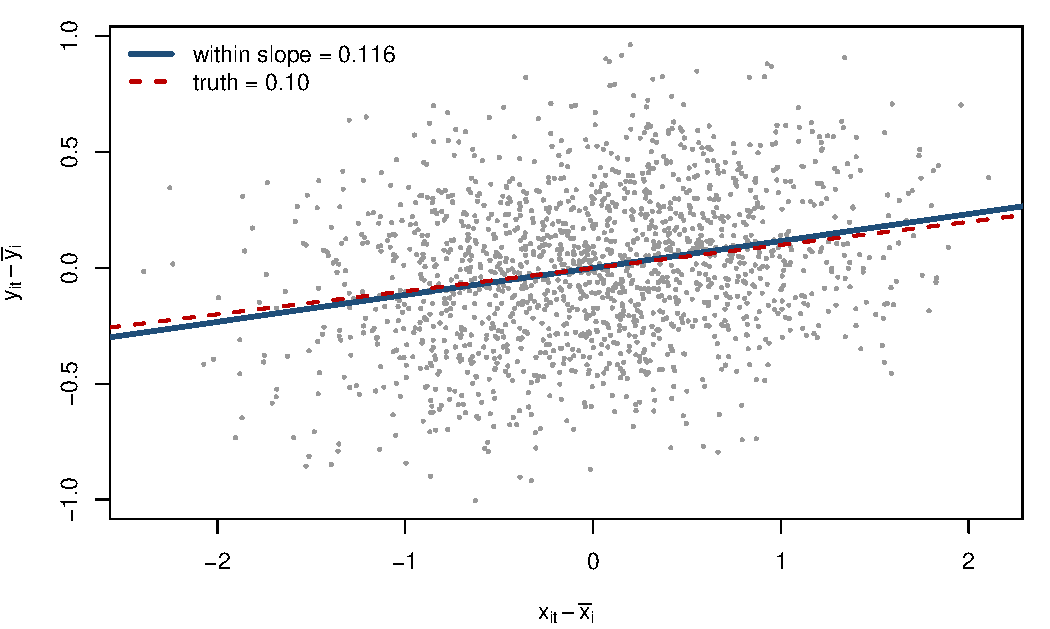
\includegraphics[width=.58\textwidth]{fig_mp_within.pdf}
\end{center}
\vspace{-.3cm}
{\small After demeaning, every firm's cloud is centered at the origin. The between-firm
variation that carried the bias is gone; what is left is the true slope, plus noise.}
\end{frame}


\begin{frame}{Estimates on the simulated panel}
\begin{center}
\begin{tabular}{lccccc}\toprule
 & Pooled OLS & First diff. & Within (FE) & Random eff. & Mundlak \\ \midrule
$\widehat\beta$ (truth $= 0.10$) & 0.246 & 0.105 & 0.116 & 0.127 & 0.116 \\
SE (cluster firm) & (0.023) & (0.013) & (0.011) & (0.011) & (0.011) \\
Coef.\ on $\bar x_i$ & & & & & 0.376 (0.054) \\
Firm FE & no & (differenced) & yes & quasi ($\hat\theta=0.72$) & no \\
$N \times T$ & 1600 & 1400 & 1600 & 1600 & 1600 \\
\bottomrule\end{tabular}

\end{center}
\medskip
\begin{itemize}
	\item Pooled OLS is off by a factor of two and a half. FE and first differences are within
	sampling error of $0.10$ (one draw; the next slide shows the distribution).
	\item Random effects and Mundlak are coming. Note the Mundlak coefficient on $\bar x_i$: it is the
	part of the pooled bias that FE removed, estimated directly.
\end{itemize}
\end{frame}


\begin{frame}{Sampling distributions (500 simulated panels)}
\begin{center}
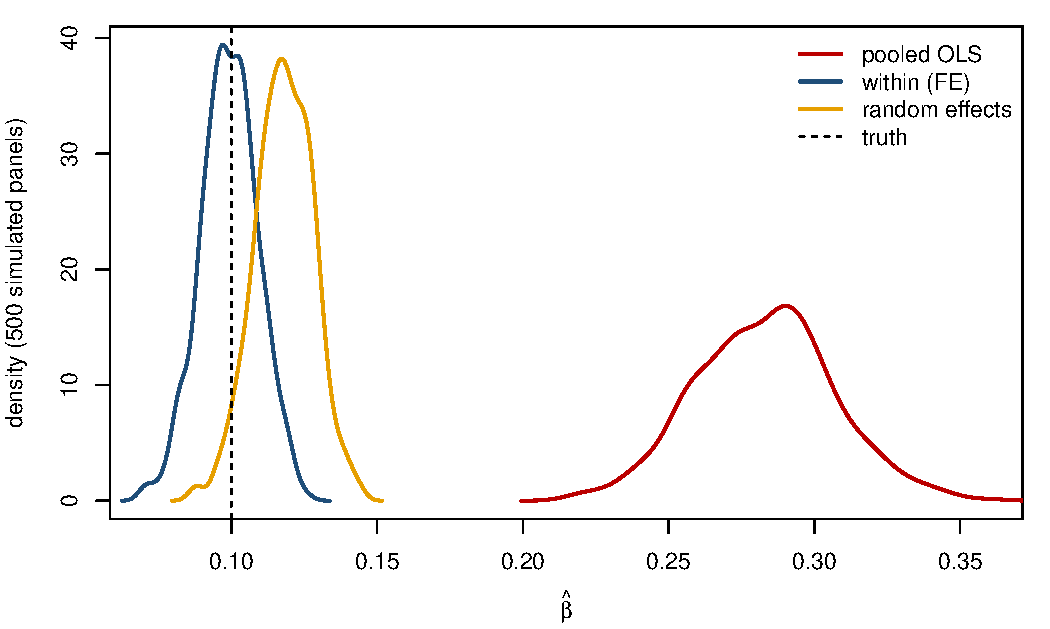
\includegraphics[width=.58\textwidth]{fig_mp_montecarlo.pdf}
\end{center}
\vspace{-.3cm}
{\small The pooled estimator is precisely wrong. FE is centered on the truth. RE is in between:
it is a weighted average of within and between information, and the between part is contaminated.}
\end{frame}


\begin{frame}{Strict exogeneity: the assumption you actually need}
For FE to be unbiased we need
\begin{align*}
	\E[\varepsilon_{it} \mid x_{i1}, \dots, x_{iT}, \alpha_i] = 0 \qquad \text{for every } t.
\end{align*}
\begin{itemize}
	\item Stronger than $\E[\varepsilon_{it} \mid x_{it}] = 0$: today's shock must be unrelated to
	\emph{past and future} $x$. Why? Demeaning mixes every period's $x$ into every period's regressor.
	\medskip
	\item What it rules out: \alert{feedback}. A firm that has a bad year ($\varepsilon_{it} < 0$)
	and responds by adopting new practices ($x_{i,t+1} \uparrow$) violates it.
	A store that sees demand jump and raises prices next week violates it.
	\medskip
	\item What it allows: $\alpha_i$ correlated with $x$ in any way at all. That is the whole appeal.
	\medskip
	\item First differences need only $\E[\Delta\varepsilon_{it} \mid \Delta x_{it}] = 0$, which is
	weaker in one direction and stronger in another; the two estimators differing a lot is itself a
	diagnostic.
\end{itemize}
\end{frame}


\begin{frame}{What FE cannot do}
\begin{itemize}
	\item \alert{Time-invariant regressors drop out.} Industry, founding year, headquarters state:
	all are absorbed by $\alpha_i$. FE cannot tell you their effect; it \emph{controls} for them.
	\medskip
	\item \alert{Identification comes from movers only.} If practices never change within a firm,
	$\tilde x_{it} = 0$ and the firm contributes nothing. Ask: who changes $x$, and why?
	\medskip
	\item \alert{Measurement error bites harder.} Demeaning removes the persistent (signal) part of
	$x$ and keeps the noisy part. Attenuation grows:
	\begin{center}
	\begin{tabular}{lccccc}\toprule
SD of measurement error in $x$ & 0 & 0.25 & 0.5 & 0.75 & 1.0 \\ \midrule
Pooled OLS ($\rho=0$, so unbiased without error) & 0.100 & 0.091 & 0.080 & 0.066 & 0.048 \\
Within (FE) & 0.100 & 0.092 & 0.071 & 0.054 & 0.038 \\
\bottomrule\end{tabular}

	\end{center}
	{\small (Here $\rho = 0$, so pooled OLS is unbiased without noise; the point is the comparison.)}
	\medskip
	\item \alert{Precision.} You are using less variation. Standard errors go up.
\end{itemize}
\end{frame}


\begin{frame}{Two-way fixed effects}
\begin{align*}
	y_{it} = x_{it}'\beta + \alpha_i + \gamma_t + \varepsilon_{it}
\end{align*}
\begin{itemize}
	\item $\gamma_t$: shocks common to everyone in period $t$. The business cycle, a platform-wide
	price change, seasonality, a pandemic.
	\medskip
	\item Estimation: demean by unit \emph{and} by period (iterate until both means are zero, which
	is what \texttt{fixest} does). Equivalent to unit dummies plus period dummies.
	\medskip
	\item Interpretation of $\beta$: the effect of a change in $x_{it}$ \emph{relative to firm $i$'s
	usual level and relative to what happened to everyone else in year $t$}.
	\medskip
	\item The workhorse of Weeks 8--9: almost every difference-in-differences you will read is a
	two-way FE regression.
\end{itemize}
\end{frame}


\begin{frame}{Random effects: the model as variance components}
Suppose $\alpha_i$ is a draw, $\alpha_i \sim (0, \sigma^2_\alpha)$, independent of $x$ and $\varepsilon$.
Write the composite error $v_{it} = \alpha_i + \varepsilon_{it}$. Then, for firm $i$:
\begin{align*}
	\Var(v_{it}) = \sigma^2_\alpha + \sigma^2_\varepsilon, \qquad
	\Cov(v_{it}, v_{is}) = \sigma^2_\alpha \ \ (t \ne s), \qquad
	\text{Corr}(v_{it}, v_{is}) = \frac{\sigma^2_\alpha}{\sigma^2_\alpha + \sigma^2_\varepsilon} \equiv \rho .
\end{align*}
\begin{itemize}
	\item Every pair of periods within a firm is \alert{equicorrelated} with correlation $\rho$.
	Stacked, $\Omega_i = \Var(v_i) = \sigma^2_\varepsilon I_T + \sigma^2_\alpha \iota\iota'$.
	\medskip
	\item Pooled OLS is unbiased under this model but inefficient: it ignores that we have
	``$N$ clusters of $T$ correlated observations,'' not $NT$ independent ones.
	\medskip
	\item The efficient estimator is GLS with this $\Omega$. That is what \alert{random effects} means.
\end{itemize}
\end{frame}


\begin{frame}{Random effects as quasi-demeaning}
GLS with $\Omega_i = \sigma^2_\varepsilon I_T + \sigma^2_\alpha\iota\iota'$ turns out to be OLS on
\emph{partially} demeaned data:
\begin{align*}
	(y_{it} - \theta\bar y_i) = (x_{it} - \theta\bar x_i)'\beta + (v_{it} - \theta\bar v_i),
	\qquad
	\theta = 1 - \sqrt{\frac{\sigma^2_\varepsilon}{\sigma^2_\varepsilon + T\sigma^2_\alpha}} .
\end{align*}
\begin{itemize}
	\item $\theta = 0$: pooled OLS. $\theta = 1$: fixed effects. RE sits in between, and the
	position is chosen by the data: how much of the variance is $\alpha$, and how many periods
	you have.
	\medskip
	\item Read the formula: as $T \to \infty$, $\theta \to 1$ and RE \emph{becomes} FE. With many
	periods per unit, the unit mean is estimated so well that GLS just removes it.
	\medskip
	\item As $\sigma^2_\alpha \to 0$, $\theta \to 0$: no firm heterogeneity, nothing to remove.
	\medskip
	\item Sketch of why: $\Omega_i^{-1/2}$ for an equicorrelated matrix is
	$\sigma_\varepsilon^{-1}\big[I_T - \theta\,\tfrac{1}{T}\iota\iota'\big]$, and applying it is
	exactly the quasi-demeaning above.
\end{itemize}
\end{frame}


\begin{frame}{How much demeaning? $\theta$ as a function of $T$}
\begin{center}
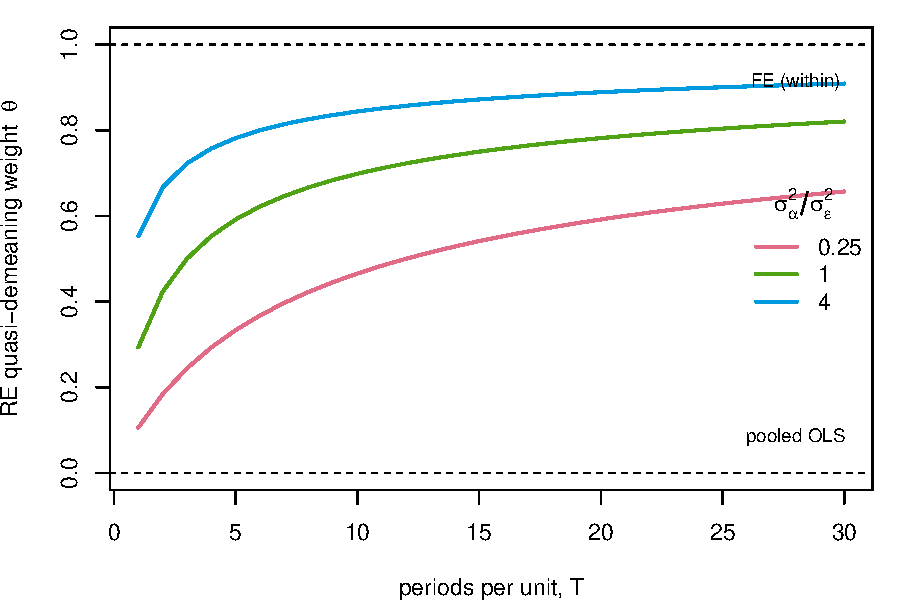
\includegraphics[width=.5\textwidth]{fig_re_theta.pdf}
\end{center}
\vspace{-.3cm}
{\small For a typical firm panel ($\sigma^2_\alpha \ge \sigma^2_\varepsilon$, $T \approx 10$), $\theta$
is already above $0.8$. RE and FE will be close in \emph{value} whenever they are both consistent; the
question is only whether RE is consistent.}
\end{frame}


\begin{frame}{Feasible GLS: estimating the variance components}
$\theta$ depends on $\sigma^2_\varepsilon$ and $\sigma^2_\alpha$, which we estimate first (Swamy--Arora):
\begin{enumerate}
	\item Run the \alert{within} regression. Its residual variance estimates $\sigma^2_\varepsilon$
	(the $\alpha_i$ are gone, so only $\varepsilon$ is left): $\hat\sigma^2_\varepsilon = \frac{\sum_{i,t}\tilde e_{it}^2}{NT - N - k}$.
	\medskip
	\item Run the \alert{between} regression: $\bar y_i$ on $\bar x_i$, one observation per firm.
	Its residual variance estimates $\sigma^2_\alpha + \sigma^2_\varepsilon / T$. Subtract:
	$\hat\sigma^2_\alpha = \hat\sigma^2_{\text{between}} - \hat\sigma^2_\varepsilon / T$ (truncate at zero).
	\medskip
	\item Form $\hat\theta$, quasi-demean, run OLS.
\end{enumerate}
\medskip
\begin{itemize}
	\item The within estimator uses only within variation; the between estimator uses only
	between variation. RE is the precision-weighted combination of the two.
	\item That sentence is also the diagnosis: if the between variation is contaminated by
	$\Cov(\bar x_i, \alpha_i) \ne 0$, RE inherits a share $(1 - \theta)$-ish of the pooled bias.
	\item The workbook implements this in a dozen lines of R; \texttt{plm} and \texttt{lme4} do it for you.
\end{itemize}
\end{frame}


\begin{frame}{RE bias as the correlation between $\alpha_i$ and $x_{it}$ grows}
\begin{center}
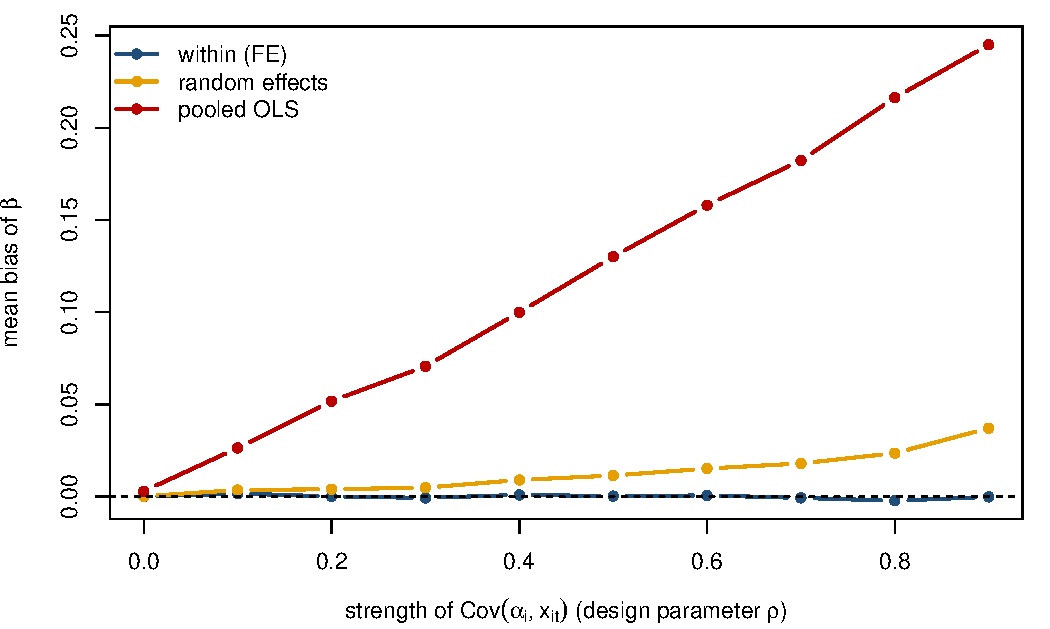
\includegraphics[width=.56\textwidth]{fig_re_bias_rho.pdf}
\end{center}
\vspace{-.3cm}
{\small FE does not care. RE is biased in proportion to the correlation, less than pooled OLS because
$\theta$ is large here ($T = 8$), but biased. Nothing about ``random'' protects you from this.}
\end{frame}


\begin{frame}{Fixed vs.\ random: what the words actually mean}
\begin{itemize}
	\item Both treat $\alpha_i$ as unobserved and $\varepsilon_{it}$ as random. The difference is
	\emph{one assumption}:
	\begin{align*}
		\text{RE: } \E[\alpha_i \mid x_{i1},\dots,x_{iT}] = 0 \qquad\qquad
		\text{FE: no restriction on } \E[\alpha_i \mid x_{i1},\dots,x_{iT}]
	\end{align*}
	\medskip
	\item Under the RE assumption both are consistent and RE is more efficient; under its failure
	only FE is consistent. Bias beats variance: economists default to FE. (Hansen: the distinction
	is about what you assume, not whether $\alpha_i$ is ``really'' random.)
	\medskip
	\item Why anyone runs RE anyway:
	\begin{itemize}
		\item you need the coefficient on a \alert{time-invariant} regressor (industry, gender, region);
		\item you believe the assumption because $x$ was \alert{randomized} across units;
		\item you care about $\alpha_i$ itself and want to \alert{shrink} noisy unit means
		(teacher effects, hospital quality, seller ratings) --- ``empirical Bayes'' is RE by another name;
		\item your field calls it a \alert{hierarchical} or \alert{mixed} model and everyone uses it.
	\end{itemize}
\end{itemize}
\end{frame}


\begin{frame}{The Hausman test}
Under the RE assumption, $\hat\beta_{FE}$ and $\hat\beta_{RE}$ estimate the same thing;
if it fails, they diverge. So test whether they differ:
\begin{align*}
	H = (\hat\beta_{FE} - \hat\beta_{RE})'\,\big[\hat V_{FE} - \hat V_{RE}\big]^{-1}(\hat\beta_{FE} - \hat\beta_{RE})
	\ \xrightarrow{d}\ \chi^2_k \quad \text{under } H_0 .
\end{align*}
\begin{itemize}
	\item The variance of the difference collapses to $V_{FE} - V_{RE}$ because RE is efficient
	under $H_0$ (the efficient estimator is uncorrelated with the difference). Neat, but fragile:
	\begin{itemize}
		\item it requires the \emph{classical} RE variance --- no clustering, no heteroskedasticity;
		\item $\hat V_{FE} - \hat V_{RE}$ need not be positive definite in finite samples;
		\item only regressors that vary within unit can be compared.
	\end{itemize}
	\medskip
	\item Rejecting says ``RE is inconsistent, use FE.'' Not rejecting says ``you could not tell'':
	with few periods RE and FE are noisy and the test has little power.
	\medskip
	\item There is a better way to run the same test.
\end{itemize}
\end{frame}


\begin{frame}{Mundlak: put $\bar x_i$ in the regression}
Model the correlation instead of assuming it away. Let
\begin{align*}
	\alpha_i = \bar x_i'\gamma + u_i, \qquad \E[u_i \mid x_{i1},\dots,x_{iT}] = 0 .
\end{align*}
Substitute:
\begin{align*}
	y_{it} = x_{it}'\beta + \bar x_i'\gamma + u_i + \varepsilon_{it} .
\end{align*}
\begin{itemize}
	\item Now $u_i$ satisfies the RE assumption by construction. Run RE (or even pooled OLS) on
	$(x_{it}, \bar x_i)$.
	\medskip
	\item Two facts (Mundlak 1978; the \alert{correlated random effects} model): the coefficient on $x_{it}$ is \emph{exactly} $\hat\beta_{FE}$,
	and $\hat\gamma$ is exactly the between-minus-within difference. The Hausman test is $H_0: \gamma = 0$.
	\medskip
	\item Advantages over the classical Hausman statistic: cluster-robust standard errors are fine;
	nothing needs to be positive definite; you can keep time-invariant regressors in the model.
\end{itemize}
\end{frame}


\begin{frame}{Both tests on the simulated panel}
\begin{center}
\begin{tabular}{lccc}\toprule
Test & Statistic & $p$-value & Verdict \\ \midrule
Hausman $(\hat\beta_{FE}-\hat\beta_{RE})^2 / (\hat V_{FE}-\hat V_{RE})$ & -4.7 & --- & undefined: $\hat V_{FE} < \hat V_{RE}$ \\
Mundlak $t$-test on $\bar x_i$ (cluster-robust) & 6.9 & $<0.001$ & reject RE \\
\bottomrule\end{tabular}

\end{center}
\medskip
\begin{itemize}
	\item The classical statistic is \emph{negative}: $\hat V_{FE} - \hat V_{RE}$ is not positive
	definite in this sample, exactly the fragility from the previous slide. (RE is inconsistent
	here, so its residual variance is inflated by the bias, and its ``efficient'' standard error is
	not smaller than FE's.) Software will either report nonsense or refuse.
	\item The Mundlak version has no such problem, rejects decisively, and came with clustered
	standard errors for free.
	\item Look back at the estimates table: the Mundlak coefficient on $x_{it}$ matched FE to three decimals.
\end{itemize}
\end{frame}


\begin{frame}{Inference: cluster by the unit}
\begin{itemize}
	\item After demeaning, the errors $\varepsilon_{it} - \bar\varepsilon_i$ are correlated within
	firm mechanically, and $\varepsilon_{it}$ itself is usually serially correlated too.
	\medskip
	\item Week 3's answer applies unchanged: cluster at the firm. Asymptotics are in $N$, the number of
	clusters, which is why ``$N$ large, $T$ small'' is the comfortable case.
	\medskip
	\item Bertrand, Duflo and Mullainathan (2004): in state-year panels with serially correlated
	outcomes, unclustered two-way FE regressions reject a true null of \emph{no effect} 45\% of the
	time at the 5\% level. Cluster.
	\medskip
	\item Cluster at the level of the fixed effect \emph{or} the level at which $x$ is assigned,
	whichever is coarser. Firm FE with a state-level policy: cluster by state.
	\medskip
	\item Few clusters (under $\approx 40$) is a separate problem; wild cluster bootstrap (Week 3).
\end{itemize}
\end{frame}


\begin{frame}{Pitfall: lagged outcomes (Nickell 1981)}
\begin{align*}
	y_{it} = \rho\, y_{i,t-1} + x_{it}'\beta + \alpha_i + \varepsilon_{it}
\end{align*}
\begin{itemize}
	\item Tempting: ``control for last year's productivity.'' Demean it:
	\begin{align*}
		(y_{it} - \bar y_i) = \rho\,(y_{i,t-1} - \bar y_i) + \dots + (\varepsilon_{it} - \bar\varepsilon_i)
	\end{align*}
	\item $\bar y_i$ contains $y_{it}$, which contains $\varepsilon_{it}$; and $\bar\varepsilon_i$
	contains $\varepsilon_{i,t-1}$, which is in $y_{i,t-1}$. Regressor and error are correlated
	\alert{by construction}.
	\medskip
	\item The bias is $O(1/T)$: it does not vanish as $N \to \infty$. With $T = 8$ and $\rho = 0.5$,
	$\hat\rho$ is biased down by roughly $0.15$, and $\hat\beta$ picks up some of the damage.
	\item Fixes (Anderson--Hsiao, Arellano--Bond) instrument $\Delta y_{i,t-1}$ with deeper lags.
	Rule for this course: no lagged dependent variable in an FE regression unless you know why.
\end{itemize}
\end{frame}


\begin{frame}{Partial pooling: no pooling, complete pooling, and the thing in between}
$60$ stores, $4$ to $64$ weeks each, true store effects $\alpha_s \sim N(0, 0.4^2)$, weekly noise SD $1$.
Three estimates of each store's effect:
\begin{itemize}
	\item \alert{No pooling}: the store's own mean (fixed effects). Unbiased; noisy when $n_s$ is small.
	\medskip
	\item \alert{Complete pooling}: the grand mean for everyone (pooled OLS). Precise; ignores that stores differ.
	\medskip
	\item \alert{Partial pooling}: $\hat\alpha_s^{PP} = \bar y + w_s(\bar y_s - \bar y)$ with
	\[
		w_s = \frac{\sigma^2_\alpha}{\sigma^2_\alpha + \sigma^2_\varepsilon / n_s} .
	\]
	The random-effects prediction, empirical Bayes, or a hierarchical model with a normal prior:
	three names, one formula. The weight is the store's signal-to-noise ratio.
\end{itemize}
\end{frame}


\begin{frame}{Partial pooling, pictured}
\begin{center}
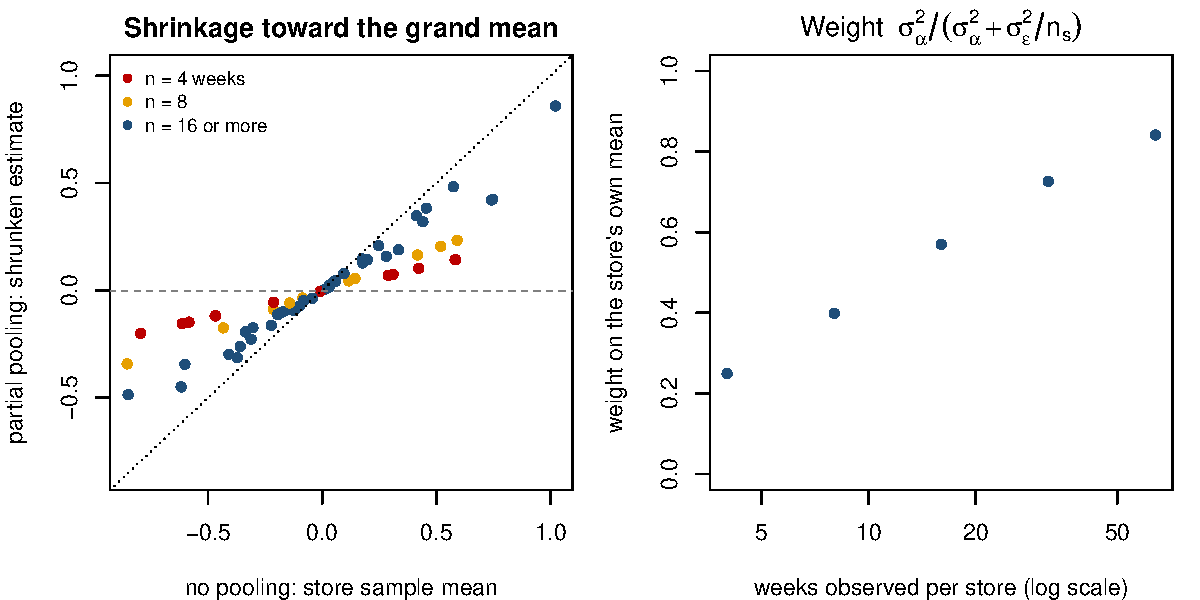
\includegraphics[width=.74\textwidth]{fig_partial_pooling.pdf}
\end{center}
\vspace{-.3cm}
{\small Left: four-week stores (red) are pulled most of the way to the grand mean; sixteen-plus-week stores keep
their own mean. Right: the weight by weeks observed. MSE against the true $\alpha_s$: no pooling $0.082$,
complete pooling $0.124$, partial pooling $0.053$.}
\end{frame}


\begin{frame}{Why marketing uses this all the time}
\begin{itemize}
	\item Partial pooling beats both extremes on mean squared error: it is the bias--variance tradeoff from
	Lecture 1b, applied sixty times with a data-driven weight.
	\medskip
	\item The \alert{ranking problem}: sort stores by sample mean and the top five include small-$n$ stores
	that got lucky; sort by the shrunken estimate and the top five are stores with enough data to be
	believed. Same logic for sellers, products, sales reps, ad creatives, teachers.
	\medskip
	\item Hierarchical Bayes in marketing (Rossi, Allenby and McCulloch 2005) is this with the prior estimated
	from the data and full posteriors instead of point estimates: customer-level coefficients in a conjoint or
	choice model are pooled toward the population with weights set by how much each customer's data can
	support. \texttt{lme4::lmer}, \texttt{brms} in R; \texttt{statsmodels.MixedLM}, \texttt{PyMC} in Python.
	\medskip
	\item When $\beta$ is the object and $\alpha_i$ a nuisance: FE. When the $\alpha_i$ themselves are the
	product: partially pool.
\end{itemize}
\end{frame}


\begin{frame}{Pitfall: when $\alpha_i$ is the object of interest}
\begin{itemize}
	\item Sometimes the fixed effect \emph{is} the estimand: which physicians have better outcomes,
	which managers add value, which sellers deliver on time.
	\medskip
	\item $\hat\alpha_i = \bar y_i - \bar x_i'\hat\beta$ is unbiased but noisy with variance
	$\approx \sigma^2_\varepsilon / T_i$. The units at the top of the ranking are disproportionately
	the ones with small $T_i$ and lucky draws.
	\medskip
	\item Shrink toward the mean in proportion to noise: the partial-pooling weight from the previous slides.
	\item Believing $\hat\alpha_i$ causally also needs strict exogeneity of the \emph{assignment}
	of units to $i$: patients are not randomly assigned to physicians (Chetty--Hendren's movers design
	is the fix).
	\item Nonlinear models (logit with firm FE) add the \alert{incidental parameters} problem:
	$\hat\beta$ is inconsistent for fixed $T$. Week 12.
\end{itemize}
\end{frame}


\begin{frame}[fragile]{In practice}
R (\texttt{fixest}):
\begin{lstlisting}
feols(y ~ x | firm + year, data = d, cluster = ~firm)          # two-way FE
d[, xbar := mean(x), by = firm]
feols(y ~ x + xbar | year, data = d, cluster = ~firm)           # Mundlak / CRE
\end{lstlisting}
Python (\texttt{pyfixest}):
\begin{lstlisting}[language=Python]
pf.feols("y ~ x | firm + year", data=d, vcov={"CRV1": "firm"})
d["xbar"] = d.groupby("firm")["x"].transform("mean")
pf.feols("y ~ x + xbar | year", data=d, vcov={"CRV1": "firm"})
\end{lstlisting}
\begin{itemize}
	\item Random effects proper: \texttt{plm(\dots, model = "random")} or \texttt{lme4::lmer(y \textasciitilde{} x + (1|firm))};
	\texttt{statsmodels.MixedLM} in Python. The workbook writes FGLS by hand so you see $\hat\theta$.
\end{itemize}
\end{frame}


\begin{frame}{Recap}
\begin{itemize}
	\item $\alpha_i$ is everything time-invariant about unit $i$. Pooled OLS is biased by
	$\Cov(x, \alpha)/\Var(x)$.
	\medskip
	\item FE removes $\alpha_i$ by demeaning (or dummies, or differencing) and needs \alert{strict
	exogeneity}: no feedback from shocks to future $x$. It uses within variation only.
	\medskip
	\item RE is GLS with equicorrelated errors, i.e.\ quasi-demeaning with weight $\theta$. It needs
	$\alpha_i \perp x$, and is biased otherwise.
	\medskip
	\item Mundlak: add $\bar x_i$. You get FE's slope, a robust Hausman test, and time-invariant
	regressors, all at once.
	\medskip
	\item Cluster by unit. Do not lag the outcome. Two-way FE is the template for next hour and next week.
\end{itemize}
\end{frame}


\begin{frame}{Workbook time}
\texttt{inclass\_session8.Rmd} (and the \texttt{pyfixest} twin):
\begin{enumerate}
	\item Reproduce the estimates table: pooled, within, FD, hand-rolled RE, Mundlak.
	\item Turn $\rho$ down to zero and up to $0.9$. Watch RE move and FE stay put.
	\item Add measurement error to $x$. Which estimator suffers more, and why?
\end{enumerate}
\end{frame}

\end{document}
